
\documentclass[12pt]{article}
\usepackage{amssymb}

%%%%%%%%%%%%%%%%%%%%%%%%%%%%%%%%%%%%%%%%%%%%%%%%%%%%%%%%%%%%%%%%%%%%%%%%%%%%%%%%%%%%%%%%%%%%%%%%%%%% 
\usepackage{amsmath}
\usepackage{amsmath,amssymb,amsthm}
\usepackage{multicol}
\usepackage{color}
\usepackage{graphicx}
\usepackage{hyperref}

\newtheorem{statement}{Statement}
\newtheorem{theorem}{Theorem}
\newtheorem{corollary}{Corollary}[theorem]
\newtheorem{lemma}{Lemma}
\newtheorem{mynote}{Note}[section]
\theoremstyle{definition}
\newtheorem{definition}{Definition}
\newtheorem{remark}{Remark}
\newtheorem{example}{Example}
\newcommand{\go}{\stackrel{\circ }{\mathfrak{g}}}
\newcommand{\ao}{\stackrel{\circ }{\mathfrak{a}}}
\newcommand{\co}[1]{\stackrel{\circ }{#1}}
\newcommand{\pia}{\pi_{\mathfrak{a}}}
\newcommand{\piab}{\pi_{\mathfrak{a}_{\bot}}}
\newcommand{\gf}{\mathfrak{g}}
\newcommand{\af}{\mathfrak{a}}
\newcommand{\aft}{\widetilde{\mathfrak{a}}}
\newcommand{\afb}{\mathfrak{a}_{\bot}}
\newcommand{\hf}{\mathfrak{h}}
\newcommand{\hfb}{\mathfrak{h}_{\bot}}
\newcommand{\pf}{\mathfrak{p}}
\newcommand{\gfh}{\hat{\mathfrak{g}}}
\newcommand{\afh}{\hat{\mathfrak{a}}}
\newcommand{\bff}{\mathfrak{b}}
\newcommand{\hfg}{\hf_{\gf}}

\theoremstyle{definition} \newtheorem{Def}{Definition}
\newcommand{\tr}{\hat\triangleright} \newcommand{\trc}{\triangleright}
\newcommand{\adk}{a^{\dagger}_{\kappa}} \newcommand{\ak}{a_{\kappa}}
\def\bF{\mbox{$\overline{\cal F}$}} \def\F{\mbox{$\cal F$}}

\begin{document}

\title{Algebraic properties of CFT coset construction and Schramm-Loewner evolution}
\author{A A Nazarov$^{1,2}$\\
  {\small $^1$ Theoretical Department, SPb State University}\\
  {\small 198904, Sankt-Petersburg, Russia}\\
  {\small$^{2}$ Chebyshev Laboratory,}\\
  {\small Department of Mathematics and Mechanics, SPb State University}\\
  {\small 199178, Saint-Petersburg, Russia}\\
  {\small email: antonnaz@gmail.com}}

\maketitle

\begin{abstract}
  Schramm-Loewner evolution appears naturally as the scaling limit of interfaces in lattice models at critical point. Critical behavior of these models can be described by minimal models of conformal field theory.

  We generalize Schramm-Loewner evolution with additional Brownian motion on Lie group to the case of direct product of two groups. We then study connection between SLE description of critical behavior with coset models of conformal field theory. In order to be consistent such construction should give minimal models for certain choice of groups. 

%%    SLE with additional Brownian motion on Lie group $G$ was proposed as generalization to WZNW models of CFT. Martingale property of SLE observables is related to Virasoro null vector conditions for CFT fields and KZ-equations for correlation functions. 
%%  
%%    Minimal models can be obtained from WZNW models by coset construction. Then it is natural to study SLE with additional Brownian motion on coset space $G/H$. We discuss algebraic properties of coset fields and correlation functions which correspond to SLE observables. 
\end{abstract}

\section{Introduction}
Schramm-Loewner evolution, introduced by Oded Schramm in papers \cite{schramm2000scaling} is 

\subsection{Schramm-Loewner evolution}
To remind of Schramm-Loewner evolution we first describe simple example.

Consider Ising model on triangular lattice on upper half plane (see Fig. \ref{fig:sle}). We impose following boundary condition: all spins are down on one half of the boundary and all spins are up on another half. Then in any configuration we get an interface delimiting two clusters and connecting zero and infinity. 

\begin{figure}[h]
  \centering{
    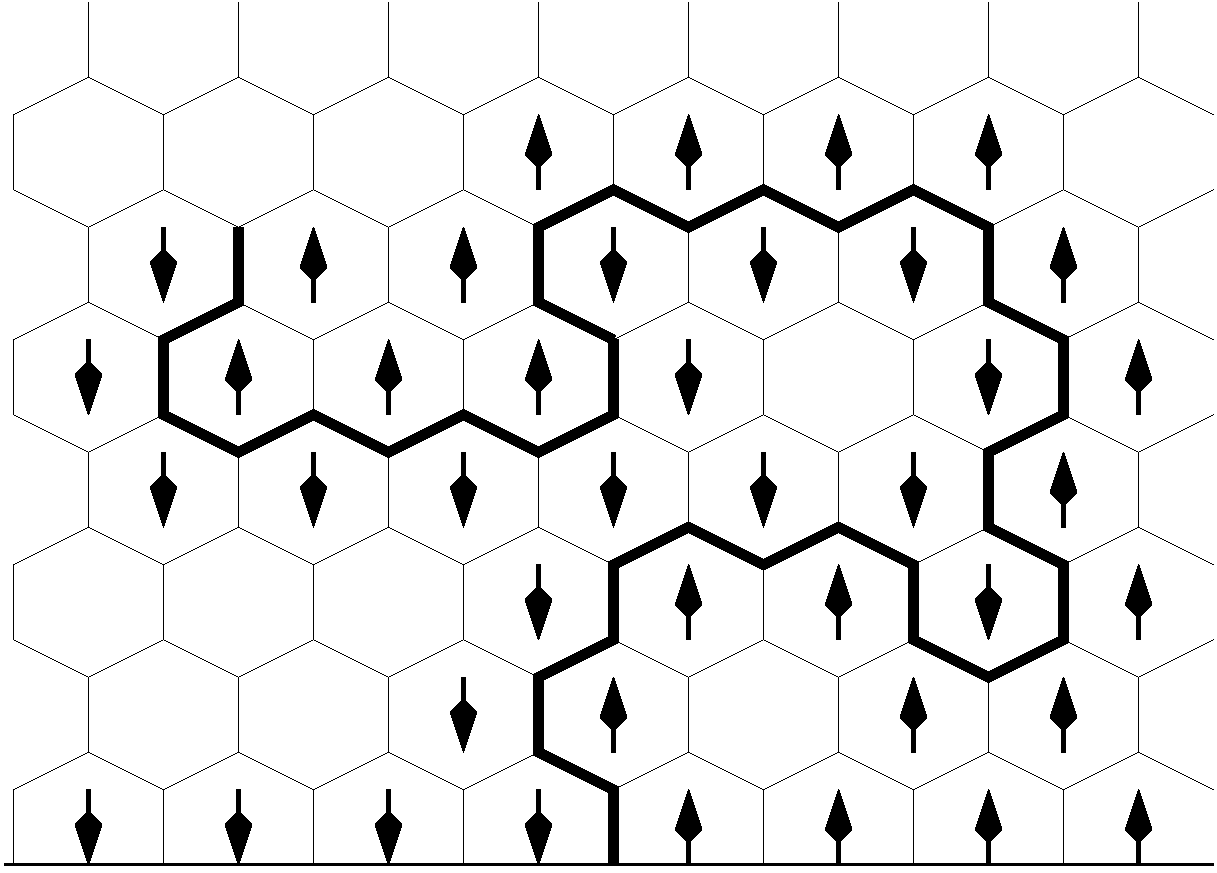
\includegraphics[height=25mm]{explore.pdf}
    \caption{SLE -- continuous limit of interfaces}}
  \label{fig:sle}
\end{figure}

Next we consider continuous limit of lattice model. Interface in random configuration of the model tends to random curve. We can think of this curve as of trace of stochastic process which satisfy some stochastic equation. 

In papers [Smirnov, Schramm ... ] it was shown that this equation is
\begin{equation*}
  \frac{\partial g_t(z)}{\partial t} = \frac{ 2}{g_t(z)-\sqrt{\kappa}\xi_{t}} \quad \text{or} \quad       d w _{t}= \frac{2dt}{w_{t} }-\sqrt{\kappa}\xi_{t}
\end{equation*}
The stochastic process which satisfy this equation is called     {\it Schramm-Loewner evolution} on the upper half-plane $\mathbb{H}$.

Here $g_{t}(z)$ is a conformal map from $\mathbb{H}_{t}=\mathbb{H}\setminus \gamma_{t}$ to $\mathbb{H}$ (see Fig. \ref{fig:sle2}).
\begin{figure}[h]
  \centering{
    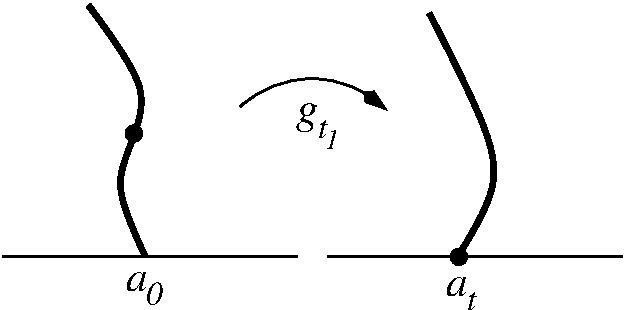
\includegraphics[width=50mm]{loewner.pdf}
    \caption{Conformal map}}
  \label{fig:sle2}
\end{figure}

Schramm-Loewner evolution provides conformally-invariant probability measure on trajectories $\gamma_{t}$ in $\mathbb{H}$.

\subsection{Correspondence between SLE and minimal models of CFT}

Now we can look at the observables in the presence of SLE trace. Expectation value of lattice observable on upper half-plane can be calculated as the sum of expectation values of this observable in presence of SLE trace up to some time $t$ multiplied by the probability of this trajectory. 

Consider lattice observable $\mathcal{O}$, then it expectation value can be calculated as
\begin{equation*}
  \prec \mathcal{O} \succ_{\mathbb{H}}=\mathbb{E}\left[\prec\mathcal{O}\succ_{\gamma_{t}}\right]=\sum_{\gamma_{t}} P\left[C_{\gamma_{t}}\right] \prec \mathcal{O} \succ_{\gamma_{t}}
\end{equation*}
Since lattice observable  $\prec \mathcal{O} \succ_{\mathbb{H}}$ does not depend on $t$, hence $\prec\mathcal{O}\succ_{\gamma_{t}}$ is a martingale.

In continuous limit lattice observable tends to CFT correlation function. Since we consider the theory with the boundary, CFT correlation function has following form:
\begin{equation*}
  \prec \mathcal{O} \succ_{\mathbb{H}_{t}}\to \mathcal{F}(\left\{z_{i}\right\})_{\mathbb{H}_{t}}=
  \frac{\left< \mathcal{O}(\{z_{i}\})\phi(z_{t})\phi^{\dagger}(\infty)\right>_{\mathbb{H}_{t}}}{\left<\phi(z_{t})\phi^{\dagger}(\infty)\right>_{\mathbb{H}_{t}}}=
  \frac{\left< ^{g_{t}}\mathcal{O}\phi(\xi_{t})\phi^{\dagger}(\infty)\right>_{\mathbb{H}}}{\left<\phi(z_{t})\phi^{\dagger}(\infty)\right>_{\mathbb{H}}}
\end{equation*}
We assume that $\mathcal{F}$ contains some set of primary fields $\phi_{\lambda_{i}}$ with conformal weights $\lambda_{i}$. Also we have boundary condition changing operators  $\phi$ at the tip of SLE trace and in the infinity.  We can use conformal map  $w(z):\mathbb{H}\setminus\gamma_{t}\to \mathbb{H}$ to rewrite this expression in upper half plane:

\begin{equation}
  \mathcal{F}(\left\{z_{i}\right\})_{\mathbb{H}_{t}}=\prod \left(\frac{\partial w(z_{i})}{\partial z_{i}}\right)^{h_{\lambda_i}} 
  \prod \left(\frac{\partial \bar w(\bar z_{i})}{\partial \bar z_{i}}\right)^{h_{\lambda^{*}_i}}
  \mathcal{F}(\left\{w_{i}, \bar w_{i}\right\})_{\mathbb{H}}
  \label{eq:1}
\end{equation}

Now we want to consider evolution of SLE trace $\gamma_{t}$ from  $t$ to $t+ dt$. First factor in right-hand-side of equation (\ref{eq:1}) gives us
\begin{equation*}
  -\frac{2h_{\lambda_{i}}}{w_{i}^{2}}\left(\frac{\partial w_{i}}{\partial z_{i}}\right)^{h_{\lambda_{i}}}.
\end{equation*}
For transformation of primary fields $\phi_{\lambda_{i}}$ we have 
\begin{equation}
  \label{eq:2}
  d\phi_{\lambda_{i}}(w_{i}) = \mathcal{G}_{i}\phi_{\lambda_{i}}(w_{i})=\left(\frac{2dt}{w_{i}}-\sqrt{\kappa} d\xi_{t}\right) \partial_{w_{i}}\phi_{\lambda_{i}}(w_{i}) 
\end{equation}
We denote generator of this transform by $\mathcal{G}_{i}$.



Continuous limit in critical point leads to CFT correlation function

Now for expectation value of martingale we have this expression.
\begin{equation*}
  \mathbb{E}\left[\prec\mathcal{O}\succ_{\gamma_{t}}\right]=    \mathbb{E}\left[\prec\mathcal{O}\succ_{\gamma_{t+dt}}\right], \quad \mathbb{E}\left[d \prec\mathcal{O}\succ_{\gamma_{t}}\right]=0
\end{equation*}

Now we use Ito calculus to calculate increment of our correlation function. It should be zero so we get the equation:
\begin{equation*}
  \left(\prod_{i=1}^{2N}\left(\frac{\partial w_{i}}{\partial z_{i}}\right)^{-h_{i}}\right)\mathbb{E}\left[d 
    \mathcal{F}_{\mathbb{H}_{t}}\right]=\left(-\sum_{i=1}^{2N}\frac{2h_{i}dt}{w_{i}^{2}}+\mathbb{E}\left[\sum_{i=1}^{2N}\mathcal{G}_{i}+\frac{1}{2}
      \sum_{i,j}\mathcal{G}_{i}\mathcal{G}_{j}\right]\right)\mathcal{F}_{\mathbb{H}}
\end{equation*}
Then use explicit form of conformal map and obtain
\begin{equation*}
  \left( \sum_{i}\left[-\frac{2h_{i}}{w_{i}^{2}} +\frac{2}{w_{i}}\partial_{w_{i}}\right]+\frac{\kappa}{2}\sum_{i,j}\partial_{w_{i}} \partial_{w_{j}}\right)\mathcal{F}(\left\{z_{i}\right\})=0
\end{equation*}

We can rewrite it as the necessary condition on b.c.c. operator $\phi$:
\begin{equation*}
  (L_{-2}-\frac{\kappa}{2}L_{-1}^{2})\phi=0 \Longrightarrow \phi \left|0\right>  \text{has level 2 null state}, \phi\sim \phi_{1,2} \;\text{or}\; \phi_{2,1}
\end{equation*}
We can see that it can be rewritten as the action of Virasoro generators. Since we have arbitrary observable, this equation is equivalent to the requirement for boundary condition changing operator to have level two null state. 
In case of minimal model we can see that boundary condition chaining operator is primary field $\phi_{1,2}$ or $\phi_{2,1}$.

\section{SLE and WZNW models}
\label{sec:sle-wzw-models}
Now we want to generalize this analysis to rational conformal field theories. First we consider Wess-Zumino-Novikov-Witten model.
\subsection{WZNW models}

 The action for this model can be written in terms of map $g:\mathbb{C}\cup \{\infty\}\sim S^{2}\to G$ from complex plane with infinity or two-sphere to some Lie group $G$:
\begin{multline}
  S=-\frac{k}{8\pi}\int d^2x\; \mathcal{K} (g^{-1}\partial^{\mu}g, g^{-1} \partial_{\mu}g)  
  \\
  - \frac{k }{24\pi^{2}} \int_{B}\epsilon_{ijk} \mathcal{K}\left(
    \tilde g^{-1}\frac{\partial \tilde g}{\partial y^i},\left[
      \tilde g^{-1}\frac{\partial \tilde g}{\partial y^j}
      \tilde g^{-1}\frac{\partial \tilde g}{\partial y^k}\right]\right) d^3y
\end{multline}
The first term is just non-linear sigma-model.

 Here $\mathcal{K}$ is Killing form on Lie algebra $\gf$ of Lie group $G$. The second term is written in terms of continuation from two-sphere $S^{2}$ to three-dimensional manifold $B$ which has two-sphere as the boundary. Since this continuation is non-unique we get the requirement for $k$ to be integer. 

Currents of this model have following form:
  \begin{eqnarray}
    J(z)= -k \partial_zg g^{-1}
    \bar J(\bar z)=k g^{-1}\partial_{\bar z}g
  \end{eqnarray}

Model possess gauge invariance under gauge transformations:
  \begin{equation*}
    g(z,\bar z)\to \Omega(z)g(z,\bar z)\bar \Omega^{-1}(\bar z),
  \end{equation*}
  where $\Omega,\;\bar \Omega \in G$.
Here $\Omega$ and $\bar \Omega$ are independent. 

If we consider infinitesimal gauge transformation $\Omega=1+\omega$ we get Ward identities:
  \begin{equation}
    \label{eq:87}
    \delta_{\omega,\bar \omega}\left< X \right>=-\frac{1}{2\pi i}\oint dz \sum\omega^a \left< J^a X\right>+
    \frac{1}{2\pi i} \oint d\bar z \sum \bar \omega^a \left< \bar J^a X\right>
  \end{equation}

 Then we can get operator product expansion for currents. 
 \begin{equation}
   \label{eq:3}
   <J\phi>\sim \dots
 \end{equation}

If we expand currents to modes
\begin{equation*}
  J^a(z)=\sum\limits_{n\in \mathbb Z}z^{n-1}J^a_n 
\end{equation*}
and use operator product expansion \eqref{eq:3} we get commutation relations of affine Lie algebra $\gfh$:
\begin{equation}
  \left[J^a_n,J^b_m\right]=\sum_c i f^{abc}J^c_{n+m}+kn\delta^{ab}\delta_{n+m,0} 
\end{equation}

This model has conformal invariance which can be seen from 
Sugawara construction. This is way to embed Virasoro algebra into the universal enveloping algebra of affine Lie algebra $\gfh$ ($Vir\subset U(\gfh)$):
\begin{equation}
  \label{eq:4}
  L_n=\frac{1}{2(k+h^v)}\sum\limits_a\sum\limits_m:J^a_m J^a_{n-m}:
\end{equation}
  
Full chiral algebra of the model is semidirect product of affine and Virasoro algebra $\gfh \ltimes Vir$. 

Its commutation relations are
  \begin{equation}
    \label{eq:92}
    \begin{aligned}
      \left[L_n,L_m\right]=(n-m)L_{n+m}+\frac{c}{12}(n^3-n)\delta_{n+m,0}\\
      \left[L_n,J^a_m\right]=-mJ^a_{n+m}
    \end{aligned}
  \end{equation}

Primary fields  $\phi_{\lambda}$ are labeled by highest weights of affine Lie algebra representations. Here we see how Virasoro and affine Lie algebra generators act on primary fields:
  \begin{equation*}
    \begin{aligned}
      & J_0^a\left|\phi_{\lambda}\right>=-t^a_{\lambda}\left|\phi_{\lambda}\right>  \quad    J^a_n\left|\phi_{\lambda}\right>=0 \quad \mbox{for}\; n>0 \\
      & L_0\left|\phi_{\lambda}\right>=\frac{1}{2(k+h^v)}\sum_aJ^a_0J^a_0\left|\phi_{\lambda}\right>=\frac{(\lambda,\lambda+2\rho)}{2(k+h^v)}\left|\phi_{\lambda}\right>=h_{\lambda} \left|\phi_{\lambda}\right>
    \end{aligned}
  \end{equation*}


\subsection{SLE and WZNW models}
Now we want to study Schramm-Loewner evolution in WZNW-models.

Similarly to minimal models we consider observable
\begin{equation*}
  \mathcal{F}(\left\{z_{i}\right\})_{\mathbb{H}_{t}}=
  \frac{\left<\phi_{\Lambda}(z_{t}) \phi_{\lambda_1}(z_{1}) \dots \phi_{\lambda_n}(z_{n}) \phi_{\lambda^{*}_1}(\bar z_{1}) \dots \phi_{\lambda^{*}_n}(\bar z_{n})
      \phi_{\Lambda^{*}}(\infty)\right>}{\left<\phi_{\Lambda}(z_{t})\phi_{\Lambda^{*}}(\infty)\right>}
\end{equation*}
Again we can use conformal map  $w(z):\mathbb{H}\setminus\gamma_{t}\to \mathbb{H}$ to rewrite it on the whole upper half-plane. 
\begin{equation*}
  \mathcal{F}(\left\{z_{i}\right\})_{\mathbb{H}_{t}}=\prod \left(\frac{\partial w(z_{i})}{\partial z_{i}}\right)^{h_{\lambda_i}} 
  \prod \left(\frac{\partial \bar w(\bar z_{i})}{\partial \bar z_{i}}\right)^{h_{\lambda^{*}_i}}
  \mathcal{F}(\left\{w_{i}, \bar w_{i}\right\})_{\mathbb{H}}
\end{equation*}

Consider evolution from $t$ to $t+dt$.
First factor gives us $-\frac{2h_{\lambda_{i}}}{w_{i}^{2}}\left(\frac{\partial w_{i}}{\partial z_{i}}\right)^{h_{\lambda_{i}}}$.

 For fields we have
\begin{equation*}
  d\phi_{\lambda_{i}}(w_{i}) = \mathcal{G}_{i}\phi_{\lambda_{i}}(w_{i})
\end{equation*}
When we consider fields we need to add random gauge transformation (random motion in $G$) to stochastic evolution \cite{bettelheim2005stochastic}, \cite{alekseev2010sle}:
\begin{equation*}
  \mathcal{G}_{i}=\left(\frac{2dt}{w_{i}}-\sqrt{\kappa} d\xi_{t}\right) \partial_{w_{i}}+\frac{\sqrt{\tau}}{w_{i}}\sum_{a=1}^{\mathrm{dim} \gf}\left(d \theta ^{a} t^{a}_{i}\right)
\end{equation*}
Since we have boundary we are working with boundary CFT so we have only half of gauge transformations due to Cardy conditions.

\subsection{SLE martingales in WZNW models}
We use Ito calculus to get the equation from martingale condition:
\begin{equation*}
  \left(-2 \mathcal{L}_{-2}+\frac{1}{2}\kappa \mathcal{L}_{-1}^{2}+\frac{1}{2}\tau\sum_{a} \mathcal{J}^{a}_{-1} \mathcal{J}^{a}_{-1}\right)        \mathcal{F}(\left\{w_{i}, \bar w_{i}\right\})_{\mathbb{H}}=0
\end{equation*}
\begin{equation*}
  \mathcal{L}_{-n}=\sum_{i}\left(\frac{(n-1)h_{\lambda_{i}}}{(w_{i}-z)^{n}}-\frac{1}{(w_{i}-z)^{n-1}}\partial_{w_{i}}\right);\quad \mathcal{J}^{a}_{{-n}}=-\sum_{i}\frac{t^{a}_{i}}{(w_{i}-z)^{n}}
\end{equation*}
Again we can rewrite it as algebraic requirement for  field  which 
correspond to boundary condition changing operator.
\begin{equation*}
  \left| \psi\right>=\left(-2 L_{-2}+\frac{1}{2}\kappa L_{-1}^{2}+\frac{1}{2}\tau\sum_{a} J^{a}_{-1} J^{a}_{-1}\right) \left|\phi_{\Lambda}\right>    
\end{equation*}
is level two null state and if we act on this state with raising operators we should get zero.
\begin{equation*}
  J^{a}_{1} \left|\psi\right>=0, J^{a}_{2}\left|\psi\right>=0.
\end{equation*}
 We use commutation relations and get equations which connects parameters of random motion with level of affine Lie algebra representation. 

We can see that $\kappa+\tau h^{v}=4$ and it is possible to derive additional relations connecting $\kappa, \tau, k$:
\begin{equation*}
  \kappa=\frac{2(h^{v}-2k)}{2h_{\Lambda}h^{v}-k},\quad \tau=\frac{8 h_{\Lambda}-2}{2h_{\Lambda}h^{v}-k}  \quad\text{for}\; k\neq 2h_{\Lambda}h^{v}
\end{equation*}
 Also we get some constraints on possible boundary condition changing operators. 
To get complete classification use Knizhnik-Zamolodchikov equations.


\section{Coset models}
\label{sec:coset-models}
Now we want to generalize analysis of correspondence between SLE and CFT even further and study coset models of conformal field theory.


\subsection{Gauged WZNW-models and coset construction}

Coset models can be realized as gauged Wess-Zumino-Novikov-Witten models. We add gauge fields  $A, \bar{A}$ taking values in Lie algebra $\af\subset \gf$ to the action:
\begin{multline*}
  S(g,A)=S_{WZNW}(g)+\\
  \frac{k}{4\pi}\int d^{2}z \left(\mathcal{K}(A, g^{-1}\bar \partial g)-\mathcal{K}(\bar A, (\partial g ) g^{-1})+\mathcal{K}(A,g^{-1}\bar A g)-\mathcal{K}(A,\bar A)\right)
\end{multline*}
Now current is
\begin{equation*}
  J_{(\gf,\af)}=-k\partial g g^{-1} -k g A g^{-1}
\end{equation*}

From Ward identities we get following expression for the product of gauge field and primary fields:
\begin{equation*}
  \left< A^{b}(z)\phi_{1}\dots \phi_{N}\right>=\frac{2}{k+2 h^{v}_{\af}}\sum_{k}\frac{\tilde{t}^{b}_{k}}{z-z_{k}}\left<\phi_{1}\dots \phi_{N}\right>
\end{equation*}
Here $h_{\af}^{v}$ is the dual Coxeter number of Lie algebra $\af$.

Remember that for WZNW current we have OPE $J_{\gf}^{a}(z)\phi_{i}(w)\sim \frac{-t^{a}_{i}\phi(w)}{z-w}$,  so we see that algebraic structure is connected with the pair of algebras $\gf$ and $\af$, such that $\afh\subset\gfh$. 

Virasoro generators are given by difference of Sugawara expressions:
\begin{equation*}
  L_{n}=L_{n}^{\gf}-L_{n}^{\af}
\end{equation*}

\subsection{Primary fields}

Primary fields are labeled by pairs of weights $(\mu,\nu)\in \hf_{\gfh}\oplus \hf_{\afh}$  of algebra and subalgebra, such that branching functions $b^{\mu}_{\nu}(q)\neq 0$. But some pairs are equivalent. This equivalence is given by the action of simple currents $(J,\tilde{J})$ such that their conformal weights are equal:  $h_{J}-h_{\tilde{J}}=0$. 

Conformal weight of primary field are equal to
\begin{multline}
  L_0\left|\phi_{(\mu,\nu)}\right>=\left(\frac{1}{2(k+h^v)}\sum_aJ^a_0J^a_0-\frac{1}{2(k+h_{\af}^v)}\sum_b \tilde{J}^b_0 \tilde{J}^b_0 \right)
  \left|\phi_{\lambda}\right>=\\
  \left(\frac{(\mu,\mu+2\rho)}{2(k+h^v)}-\frac{(\nu,\nu+2\rho_{\af})}{2(k+h^v)}\right)\left|\phi_{(\mu,\nu)}\right>
\end{multline}

%% So $G/A$-coset theory is related to $\gf\oplus \bar{\af}$-theory.

It is possible to obtain analogues of KZ-equations:
\begin{equation*}
  \left\{\frac{1}{2}\partial_{i} + \sum_{i\neq j}^{N}\left(\frac{t^{a}_{i}t^{a}_{j}}{k+h^{v}}-\frac{\tilde t^{b}_{i}\tilde t^{b}_{j}}{k+h^{v}_{\af}}\right)\frac{1}{z_{i}-z_{j}}\right\} \left<\phi_{1}(z_{1})\dots \phi_{N}(z_{N})\right>=0
\end{equation*}

\subsection{SLE on coset space}
Consider gauge transformation in gauged WZNW model:
\begin{eqnarray*}
  \delta \phi_{i}=(\epsilon_{L}^{a} t^{a}_{i}+\epsilon^{b}_{R}\tilde{t}^{b})\phi_{i}\\
  \delta A = -\partial \epsilon_{R}-[\epsilon_{R},A]
\end{eqnarray*}
Here $\epsilon_{L}, \epsilon_{R}$ are arbitrary holomorphic functions $\bar\partial\epsilon_{L,R}=0$. 
For  $\gf\oplus \af$ WZNW-model we can write SLE generator of primary field transformation under stochastic evolution as
\begin{equation*}
  \mathcal{G}_{i}=\left(\frac{2dt}{w_{i}}-\sqrt{\kappa} d\xi_{t}\right) \partial_{w_{i}}+\frac{\sqrt{\tau}}{w_{i}}\left(\sum_{a=1}^{\mathrm{dim} \gf}\left(d \theta ^{a} t^{a}_{i}\right)+\sum_{b=1}^{\mathrm{dim} \af}\left(d \tilde{\theta} ^{b} \tilde{t}^{b}_{i}\right)\right)
\end{equation*}
%% \begin{equation*}
%%   \mathcal{G}_{i}^{L,R}=\left(\frac{2dt}{w_{i}}-\sqrt{\kappa} d\xi_{t}\right) \partial_{w_{i}}+\frac{\sqrt{\tau}}{w_{i}}\left(\sum_{a=1}^{\mathrm{dim} \gf}\left(d \theta ^{a} t^{a}_{i}\right)\pm\sum_{b=1}^{\mathrm{dim} \af}\left(d \tilde{\theta} ^{b} \tilde{t}^{b}_{i}\right)\right)
%% \end{equation*}

and get martingale condition
\begin{equation*}
  \left(-2 \mathcal{L}_{-2}+\frac{1}{2}\kappa \mathcal{L}_{-1}^{2}+\frac{\tau}{2}\left( \sum_{a} \mathcal{J}^{a}_{-1} \mathcal{J}^{a}_{-1}-
      \sum_{b}\tilde{\mathcal{J}}^{b}_{-1} \tilde{\mathcal{J}}^{b}_{-1}\right)\right)        \mathcal{F}_{\mathbb{H}}=0
\end{equation*}

which can be rewritten as the requirement for
\begin{equation*}
  \psi=\left(-2L_{-2}+\frac{1}{2}\kappa L_{-1}^{2}+\frac{1}{2}\tau \left(\sum_{a=1}^{\mathrm{dim}\gf}J^{a}_{-1}J^{a}_{-1}-\sum_{b=1}^{\mathrm{dim}\af}\tilde{J}^{b}_{-1}\tilde{J}^{b}_{-1}\right)\right) \phi_{(\Lambda,\Gamma)}
\end{equation*}
to be level two null-field.

We can compare this result with the simplest possible coset model $su(2)/u(1)$ --  parafermion theory.

\subsection{Semisimple Lie algebras and coset construction}
\label{sec:semis-lie-algebr}

It is well known that unitary minimal models with central charge $c=1-\frac{6}{m(m+1)}$ can be obtained from coset construction starting with $su(2)_{m}\oplus su(2)_{1}$ WZW-model and factorizing it by $su(2)_{m+1}$. Here lower index represents level of affine Lie algebra representation. 

In this case the dimension of Lie algebra $\gf=su(s)\oplus su(2)$ is 6, dual Coxeter number $h^{v}=2+2=4$. 


\begin{equation}
  \left| \psi\right>=\left(-2 L_{-2}+\frac{1}{2}\kappa L_{-1}^{2}+\frac{1}{2}\tau\sum_{a} J^{a}_{-1} J^{a}_{-1}\right) \left|\phi_{\Lambda}\right>    
\label{eq:6}
\end{equation}

For semisimple Lie algebra $\gf=\gf_{1}+\gf_{2}$ with generators $J^{a}$ and $\tilde{J}^{b}$ correspondingly we can more explicitly write the relation \eqref{eq:6} as 

\begin{equation*}
  \left| \psi\right>=\left(-2 L_{-2}+\frac{1}{2}\kappa L_{-1}^{2}+\frac{1}{2}\tau\left(\sum_{a} J^{a}_{-1} J^{a}_{-1}+\sum_{b}\tilde{J}^{b}_{-1}\tilde{J}^{b}_{-1}\right) \right) \left|\phi_{\Lambda}\right>    
\end{equation*}

This vector should be null vector of level two, so $L_{2}\left|\psi\right>=L_{1}\left|\psi\right>=0$. Then we get following algebraic relations for semisimple Lie algebra:
\begin{equation}
  \label{eq:7}
  \left( 3\kappa h_{\Lambda} +\frac{1}{2} \tau (k_{1} \mathrm{dim} \gf_{1}+k_{2}\mathrm{dim} \gf_{2}) -8 h_{\Lambda} - c\right)\phi_{\Lambda}=0
\end{equation}
SLE and factorization by equivalence relations. 

\subsection{Parafermions}

$\mathbb{Z}(N)$ parafermions are equivalent to $SU(2)_{N}/U(1)$ coset theory.

It is well-known that parafermionic field can be written as product of $su(2)$-primary field and vertex operator of bosonic field. 
\begin{equation*}
  \Phi^{j}=\phi_{j}(z) \exp\left( -i \frac{j}{\sqrt{N}}\phi(z)\right)
\end{equation*}
where $\phi_{j}(z)$ is field of $SU(2)$-WZNW model with spin $j$, $\phi(z)$ -- $U(1)$ bosonic field.

For parafermionic current we have
\begin{equation*}
  \Psi^{\pm}=\frac{1}{\sqrt{N}} J^{\pm}\exp\left(\mp i \frac{1}{\sqrt{N}}\phi(z)\right)
\end{equation*}
%% Its action in terms of primary fields of $su(2)\oplus u(1)$ WZNW-model is equivalent to $J^{\pm}\pm \tilde{J}^{\pm}$.
%% !!! TODO
Martingale condition can be rewritten as
\begin{equation*}
  \left(-2 L_{-2}+\frac{\kappa}{2}L_{-1}^{2}+\frac{\tau}{2}\left[\Psi^{+}_{-1}\Psi^{-}_{-1}+\Psi^{-}_{-1}\Psi^{+}_{-1}\right]\right) \left|\Phi\right>=0
\end{equation*}
which coincides with the result of Santachiara [arXiv:0705.2749].



\subsection{Next steps}

Next steps in the study of SLE martingales for coset models  are the following. 

%At first we act on $  \psi=\left(-2L_{-2}+\frac{1}{2}\kappa L_{-1}^{2}+\frac{1}{2}\tau \left(\sum\limits_{a=1}^{\mathrm{dim}\gf}J^{a}_{-1}J^{a}_{-1}+\sum\limits_{b=1}^{\mathrm{dim}\af}\tilde{J}^{b}_{-1}\tilde{J}^{b}_{-1}\right)\right) \phi_{(\Lambda,\Gamma)}$ with  raising operators $J^{(a,b)}_{1}, J^{(a,b)}_{2}$ and get relations which connects level of representation and parameters of random motion $\kappa, \tau$. 
% !!! This is wrong !!!
% We can act by Sugawara generators 

Then we use Knizhnik-Zamolodchikov equations to rewrite the relations in simpler form and get conditions on possible boundary condition changing operators. 

Boundary states in coset models were actively studied. One of the ideas is to consider direct sum WZNW-model and use equivalence relations. This study is essentially the study representation of fusion algebra, Verlinde formula is one of key ingredients in this study. So we hope to compare the classification of boundary states obtained in this way with our condition on boundary condition changing operator. 

\section{Conclusion}
\label{sec:conclusion}

Now we see that it is possible to match SLE observables and CFT correlation functions. Martingale conditions can be seen as the constraints on possible Verma modules of affine Lie algebra corresponding to boundary condition changing operator. These Verma modules must have level two null state. 

We can use primary fields of direct sum WZNW model and equivalence relations to study coset models. 

Martingale conditions should be compared with the classification of boundary states with other methods.

\bibliography{bibliography}{}
\bibliographystyle{utphys}

\end{document}
%%% Local Variables: 
%%% mode: latex
%%% TeX-master: t
%%% End: 
